\documentclass[conference]{IEEEtran}

\usepackage{cite}
\usepackage{amsmath,amssymb,amsfonts}
\usepackage{algpseudocode}
\usepackage{algorithm}
\usepackage{graphicx}
\usepackage{textcomp}
\usepackage{xcolor}
\def\BibTeX{{\rm B\kern-.05em{\sc i\kern-.025em b}\kern-.08em
    T\kern-.1667em\lower.7ex\hbox{E}\kern-.125emX}}
\begin{document}

\title{Forest Cover Classification\\

}

\author{\IEEEauthorblockN{David Nicolay}
\IEEEauthorblockA{\textit{Department of Computer Science} \\
\textit{Stellenbosch University}\\
Stellenbosch, South Africa \\
26296918@sun.ac.za}
}

\maketitle

\begin{abstract}
This document is a model and instructions for \LaTeX.
This and the IEEEtran.cls file define the components of your paper [title, text, heads, etc.]. *CRITICAL: Do Not Use Symbols, Special Characters, Footnotes, 
or Math in Paper Title or Abstract.
\end{abstract}

\begin{IEEEkeywords}
component, formatting, style, styling, insert.
\end{IEEEkeywords}

\section{Introduction}
introooo TODO remove
``Fig.~\ref{fig}'', even at the beginning of a sentence.

\begin{table}[htbp]
\caption{Table Type Styles}
\begin{center}
\begin{tabular}{|c|c|c|c|}
\hline
\textbf{Table}&\multicolumn{3}{|c|}{\textbf{Table Column Head}} \\
\cline{2-4} 
\textbf{Head} & \textbf{\textit{Table column subhead}}& \textbf{\textit{Subhead}}& \textbf{\textit{Subhead}} \\
\hline
copy& More table copy$^{\mathrm{a}}$& &  \\
\hline
\multicolumn{4}{l}{$^{\mathrm{a}}$Sample of a Table footnote.}
\end{tabular}
\label{tab1}
\end{center}
\end{table}

\begin{figure}[htbp]
\centerline{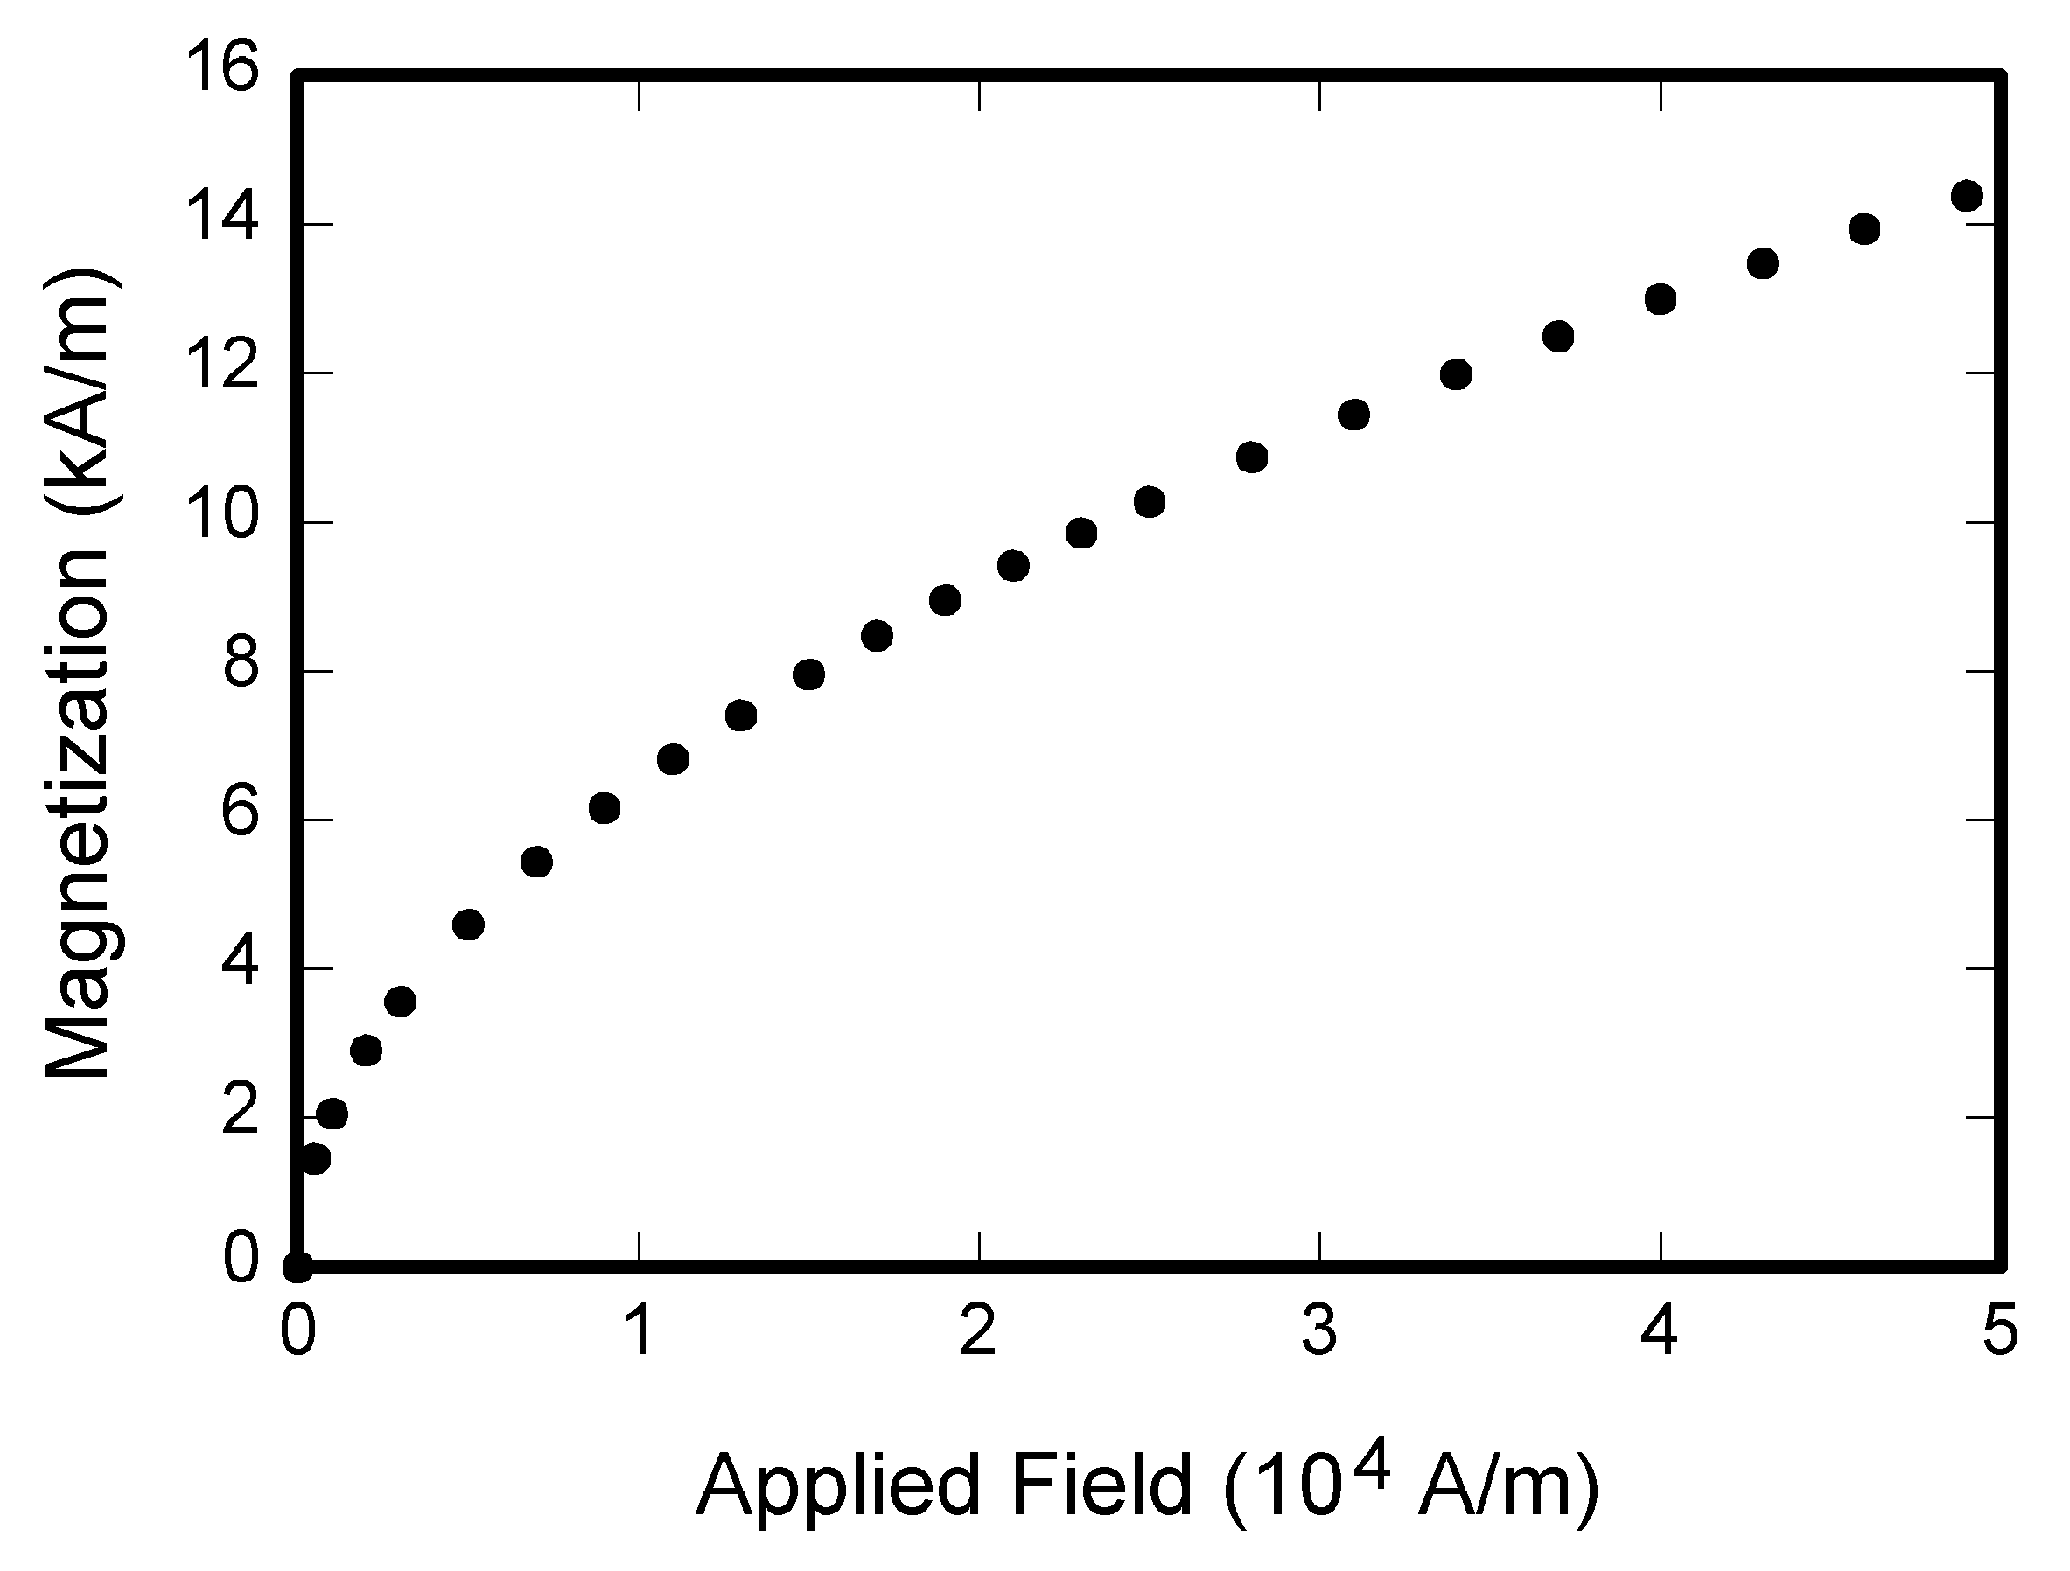
\includegraphics{fig1.png}}
\caption{Example of a figure caption.}
\label{fig}
\end{figure}

Figure Labels: Use 8 point Times New Roman for Figure labels. Use words 
rather than symbols or abbreviations when writing Figure axis labels to 
avoid confusing the reader. As an example, write the quantity 
``Magnetization'', or ``Magnetization, M'', not just ``M''. If including 
units in the label, present them within parentheses. Do not label axes only 
with units. In the example, write ``Magnetization (A/m)'' or ``Magnetization 
\{A[m(1)]\}'', not just ``A/m''. Do not label axes with a ratio of 
quantities and units. For example, write ``Temperature (K)'', not 
``Temperature/K''.

\section{Introduction}
\section{Background}

\subsection{k-nearest Neighbours (kNN)}
The nearest neighbour algorithm is an example of instance-based learning where the prediction for an instance is made by comparing the instance to similar training instances. This is a lazy learning approach since we delay processing training data until prediction is needed. Since kNN is also similarity-based, it is non-parametric, which means that it does not learn a mapping from the input space to the output space.

The k-nearest neighbour algorithm is presented in Algorithm~\ref{alg:knn} which explains that we calculate the distance from each data point in our training dataset to the distance. From there, we choose the closed \textit{k} observations and perform inference. In a classification context we may perform majority voting to determine the class, in a regression context we use the mean or median of the \textit{k} nearest observations.

In order to use the algorithm we need to define a value of \textit{k} which decides the number of nearest neighbour instances to consider when predicting. Choosing a value a low value for \textit{k} results in a high variance, but low bias leading to an unstable model which tends to overfit. Choosing a large value for \textit{k} results in a smaller variance, but high bias, leading to a more stable model which tending to underfit. Measures such as \textit{k}-fold cross validation assist in the selection of a value of \textit{k}.

\begin{algorithm}[htbp]
\caption{k-Nearest Neighbors Algorithm}
\label{alg:knn}
\begin{algorithmic}
\Function{kNN}{$D, x, k$}
\ForAll{$x' \in D$}
\State $d = \text{distance}(x, x')$
\EndFor
\State sort($d$)
\State $S = $ set of $k$ patterns in $D$ closest to $x$
\State \Return class as majority class in $S$
\EndFunction
\end{algorithmic}
\end{algorithm}
\noindent
\textbf{Notation:} $D$ denotes the training dataset, $x$ is the query instance, $k$ is the number of nearest neighbours, and $\text{distance}(\cdot)$ is a distance metric (e.g., Euclidean distance).


\subsection{Classification Trees}
Classification trees represent a fundamental approach in supervised machine learning for predictive modelling, where the learned model forms a hierarchical tree structure with non-terminal nodes representing decisions on descriptive features and terminal leaf nodes representing target feature predictions \cite{quinlan1993c45}. A classification tree is a type of decision tree where leaf nodes represent different discrete classes.

Classification trees employ recursive partitioning where a training dataset is systematically divided into increasingly homogeneous subsets based on feature values. It uses a greedy strategy to select the feature to partition upon at each split that maximises information gain \cite{kelleher2020fundamentals}. The information gain criterion, derived from Shannon's entropy measure, quantifies the reduction in uncertainty achieved by partitioning the data according to a specific feature test.
Formally, given a dataset $D$ with $M$ different classes, the entropy is calculated as:

\[
H(D) = -\sum_{m=1}^{M} p(y_m) \log_{M} p(y_m)
\]

where $p(y_m)$ represents the probability of class $y_m$ occurring in $D$. When the dataset is partitioned on feature $\alpha$ into $O$ outcomes, the information gain is computed as:

\[
\text{gain}(\alpha) = H(D) - H_\alpha(D)
\]

where 

\[
H_\alpha(D) = \sum_{o=1}^{O} p_o \, H(D_o)
\]

represents the weighted entropy after the split.

Since we recursively partition until either a stopping condition is satisfied or all subsets are homogeneous, classification trees inherently lead to overfitting, as the algorithm attempts to perfectly classify all training instances, often creating overly complex trees that capture noise rather than underlying patterns \cite{quinlan1993c45}. To remedy this, post-pruning techniques are used to remove branches that do not improve generalisation performance.

Classification trees can naturally handle both categorical and numerical features. Classification tree induction algorithms can cope with missing values. Unfortunately, classification trees exhibit an axis-aligned bias which restricts decision boundaries to be parallel to feature axes.

\subsection{Expectations With Respect to Data Quality Issues}
Since kNN relies heavily on distance metrics, it will be severely impacted by missing values since it cannot compute meaningful distances between points. This can however be handled by ignoring the missing values in the distance calculation and scaling up the weight of the non-missing descriptive features. The kNN algorithm can actually be used as an imputer itself as well. If nothing is done the algorithm will either fail or give biased distances. Classification trees on the other hand handle missing values more gracefully. Classification trees can adjust the gain ratio calculation 
\[
\text{gainRatio}(x) = (1 - F) \times \big( H(D) - H_x(D) \big)
\]

\text{where } F \text{ is the fraction of missing patterns.}



With regards to the Facet feature being correlated with the Aspect feature, kNN will be moderately impacted since the distance calculation used will overweight certain areas of similarity. There is no built in mechanism to handle feature correlation as a data issue. Classification trees will be minimally impacted since trees naturally handle correlated features through the feature selection process involving the gain ratio/information gain. This means that the classification tree induction will likely select one feature and ignore the correlated redundant one.

Concerning the Inclination feature only containing noisy values, the impact on the kNN algorithm will depend on the value of \textit{k} since higher values are more sensitive to noise and lower values are more robust to noise. However, since there are many predictive features the value won't dominate the distance calculation. Classification trees are robust to noise and will handle it through pruning. The noisy patterns will end up in small leaf nodes as the model overfits and post-pruning removes these leaves. The noise becomes a minority and does not affect majority class prediction.

Since kNN employs distance measures which are often sensitive to outliers since the distance can be seriously skewed even if only one feature is outlying. For small values of \textit{k} outliers are unlikely to be nearest neighbours and will therefore have limited influence. For large values of \textit{k} the outliers will also have limited influence due to majority voting. Cumulatively, outliers will have a moderate impact on the kNN algorithm. Classification trees are robust to outliers since they handle them in a similar way to noise. Outliers are first isolated in small leaf nodes during induction. Pruning removes leaves which contain outliers which results in outliers becoming a minority in combined larger subsets. This makes decision trees robust to outliers.

The kNN algorithm will be severly impacted from features with numeric ranges that differ significantly from one another since features with large ranges dominate distance calculations. For example, if one feature takes on the value of 0 or 1 and another takes on the value of 0 or 100 000, the second will overwhelm the distance calculation. Without normalisation, the kNN algorithm will be unreliable. Classification trees have a natural robustness to different feature scales and therefore will be minimally impacted. This stems from trees using individual feature values for splitting thresholds.

The mixed data types will affect the kNN algorithm since it requires special handling for mixed types such as using the Gower's similarity with different similarity measures for different types. However, in this dataset since there are two categorical variables with the first encoded over four columns and the second over 40 and 13 numeric features there can be a distance bias toward the numeric features. Euclidean distance assumes features are continuous, but the categorical features are encoded as zero or one. Classification trees naturally handle mixed data types since they directly compare categorical features against each other for splitting, and the splitting is simply decided off information gain.

The impact of the Water Level feature having a cardinality of one will be none at all for kNN. It will only contribute the the distance calculation unnecessarily and be a computational waste. Since all observations have the same value, all the distance measures will be equally skewed, resulting in no impact at all. The classification tree will never select this feature during tree indication since there is zero information gain because all values are identical. Therefore, classification trees naturally handle this issue and it will have no impact.

The Observation ID unique feature will have a sever impact on kNN since each instance appears maximally different from all others on this feature. The problem is that this dominates distance calculations making all instances seem dissimilar. It breaks the fundamental assumption of similarity-based learning. Classification trees will overfit severely since each unique value would create a separate branch. The information gain maximisation favours features with many outcomes so the result will be an extremely busy tree with poor generalisation.

The skewed class distribution impact on kNN depends on the value of \textit{k}, since a smaller \textit{k} is more robust to class imbalance whilst a large \textit{k} results in the majority class dominating the predictions. Methods such as SMOTE must be considered. The impact of classification trees is moderate since they are sensitive to skewed distributions. The minority class instances result in small leaves which are likely to be pruned, then the combined instances will be classification as a majority class. This results in poor minority class recognition.

\section{Methodology}
\section{Empirical Procedure}
\section{Research Results}
\section{Conclusion}
\section*{References}

Please number citations consecutively within brackets \cite{eason1955}. The 
sentence punctuation follows the bracket \cite{maxwell1892}. Refer simply to the reference 
number, as in \cite{jacobs1963}---do not use ``Ref. \cite{jacobs1963}'' or ``reference \cite{jacobs1963}'' except at 
the beginning of a sentence: ``Reference \cite{jacobs1963} was the first $\ldots$''

Number footnotes separately in superscripts. Place the actual footnote at 
the bottom of the column in which it was cited. Do not put footnotes in the 
abstract or reference list. Use letters for table footnotes.

Unless there are six authors or more give all authors' names; do not use 
``et al.''. Papers that have not been published, even if they have been 
submitted for publication, should be cited as ``unpublished'' \cite{elissa}. Papers 
that have been accepted for publication should be cited as ``in press'' \cite{nicole}. 
Capitalize only the first word in a paper title, except for proper nouns and 
element symbols.

For papers published in translation journals, please give the English 
citation first, followed by the original foreign-language citation \cite{yorozu1987}.

\bibliographystyle{IEEEtran}
\bibliography{references}

\end{document}
